%!TEX TS-program = xelatex
%!TEX encoding = UTF-8 Unicode

\documentclass[12pt,a4paper,oneside]{book}
\usepackage{nfu-thesis}

%% ================================================================
%% 論文基本資料：一般使用者主要修改這一區即可
%% ================================================================
\NFUSetup{
  mainfont     = {Times New Roman},
  cjkfont      = {TW-Kai},
  universityen = {National Formosa University},
  universityzh = {國立虎尾科技大學},
  collegeen    = {College of Management},
  collegezh    = {管理學院},
  instituteen  = {Department of Industrial Management},
  institutezh  = {工業管理系工業工程與管理碩士班},
  fielden      = {Industrial Engineering and Management},
  degreezh     = {碩士},
  degreeen     = {Master of Science},
  classzh      = {論文},
  classen      = {Thesis},
  titleen      = {English Title},
  titlezh      = {中文題目},
  studenten    = {your name},
  studentzh    = {你的名字},
  advisoren    = {advisor's name},
  advisorzh    = {指導教授姓名},
  yearen       = {2027},
  yearzh       = {116},
  monthen      = {July},
  monthzh      = {7},
  watermark    = {watermark_nfu.jpg},
  approvalpdf  = {approval.pdf}
}

\XeTeXlinebreaklocale "zh"
\XeTeXlinebreakskip = 0pt plus 1pt
\tracinglostchars=0

\begin{document}
\hypersetup{pageanchor=false}
\pagenumbering{gobble}

%% ── 封面 ────────────────────────────────────────────────────────────────
\makeNFUCover

%% ── 書背（可選）：先獨立編譯 bookspine.tex 產生 bookspine.pdf ────────────
% \clearpage
% 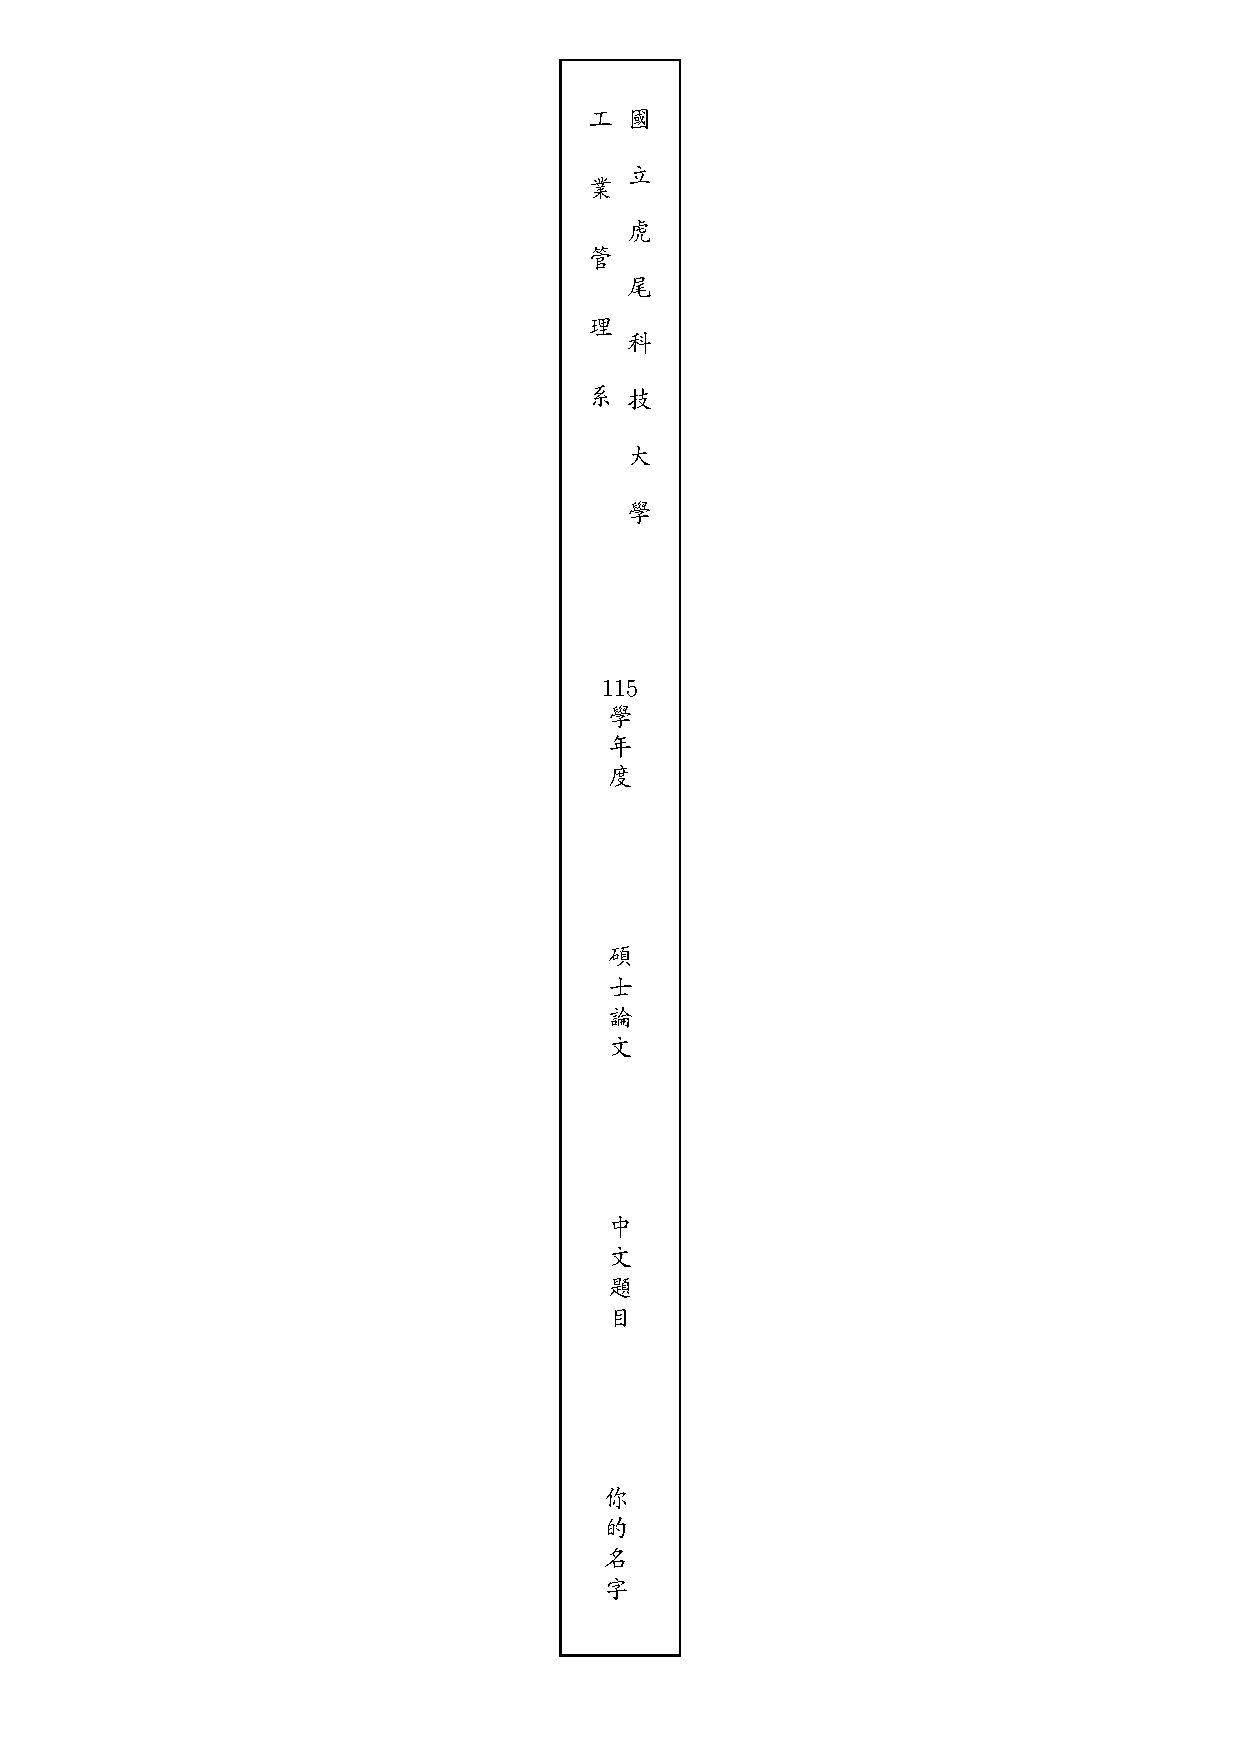
\includepdf{bookspine.pdf}
% \clearpage

%% ── 書名頁 ──────────────────────────────────────────────────────────────
\makeNFUTitlePage

%% ── 口試委員審定書（PDF）────────────────────────────────────────────────
\makeNFUApprovalPage

%% ── 授權書（PDF）────────────────────────────────────────────────



%% ── 前置頁：小寫羅馬頁碼 ────────────────────────────────────────────────
\NFUFrontMatter
\NFUWatermarkOn

%% ----------- 中文摘要 ----------------------
\begin{NFUAbstractZH}
這是摘要的內容......。\\
\newline
\noindent
關鍵字：關鍵詞、關鍵詞
\end{NFUAbstractZH}
%% ---------- English Abstract ----------------
\begin{NFUAbstractEN}
This is abstract.\\

\noindent
Keywords: keyword, keyword, keyword
\end{NFUAbstractEN}


%% ---------- 誌謝 ---------------
\begin{NFUAcknowledge}
誌謝內容......。
\end{NFUAcknowledge}

%% ── 目錄、表目錄、圖目錄 ──────────────────────────────────────────────
\clearpage
\tableofcontents
\clearpage
\listoftables
\clearpage
\listoffigures

%% ── 正文：阿拉伯頁碼 ────────────────────────────────────────────────────
\NFUMainMatter
\counterwithin{table}{chapter}
\counterwithin{figure}{chapter}
\counterwithout{equation}{chapter}


%% ==================== introduction ====================
\chapter{緒論}
\label{c:intro}

\section{研究動機}

文獻\cite{test2021}指出... ...。測試文字測試文字測試文字測試文字測試文字測試文字測試測試文字測試文字測試文字測試文字測試文字測試文字測試

測試文字測試文字測試文字測試文字測試文字測試文字測試文字測試文字測試文字測試文字測試文字測試文字測試文字測試文字測試文字測試文字測試文字測試文字測試文字測試文字測試文字測試文字測試文字測試文字測試文字測試文字測試文字測試文字測試文字測試文字

\section{研究背景}
\subsection{測試測試}

測試文字測試文字測試文字測試文字測試文字測試文字測試測試文字測試文字測試文字測試文字測試文字測試文字測試

\section{研究目標}

\begin{enumerate}
\item 測試 
\item 測試 
\item 測試
\item 測試
\end{enumerate}

\section{研究問題}
整合上述，測試文字測試文字測試文字測試文字測試文字測試文字測試文字測試文字測試文字測試文字測試文字測試文字測試文字測試文字測試文字。

\section{研究重要性} 

測試文字測試文字測試文字測試文字測試文字測試文字測試文字測試文字測試文字測試文字測試文字測試文字測試文字測試文字測試文字。


%% ==================== related ====================
\chapter{文獻探討}
\label{c:related}

\section{測試}

測試文字測試文字測試文字\cite{test2018,test2019}。

測試文字測試文字測試文字測試文字測試文字測試文字測試文字測試文字測試文字測試文字測試文字測試文字測試文字測試文字測試文字測試文字測試文字測試文字測試文字測試文字測試文字測試文字測試文字測試文字測試文字測試文字測試文字測試文字測試文字測試文字測試文字測試文字測試文字測試文字測試文字測試文字測試文字測試文字測試文字測試文字測試文字測試文字測試文字測試文字測試文字測試文字測試文字測試文字。

測試文字測試文字測試文字測試文字測試文字測試文字測試文字測試文字測試文字測試文字測試文字測試文字測試文字測試文字測試文字測試文字測試文字測試文字測試文字測試文字。

\noindent
無縮排測試文字

\begin{figure}[!htb]
\centering

\subfloat[文字]{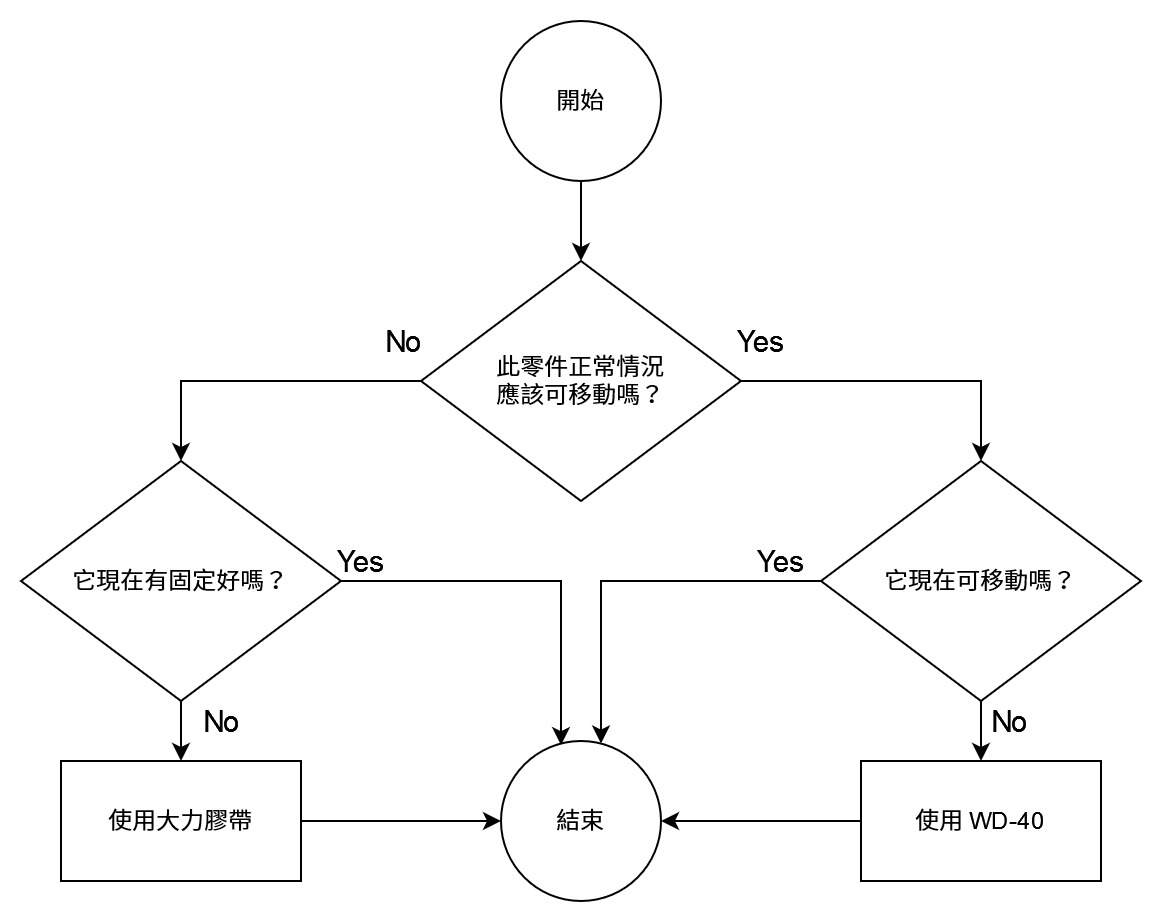
\includegraphics[width=.95\columnwidth]{debug.jpg}} \\
\subfloat[]{
\includegraphics[width=.45\columnwidth]{watermark_nfu.jpg}}\hspace{5pt}
\subfloat[]{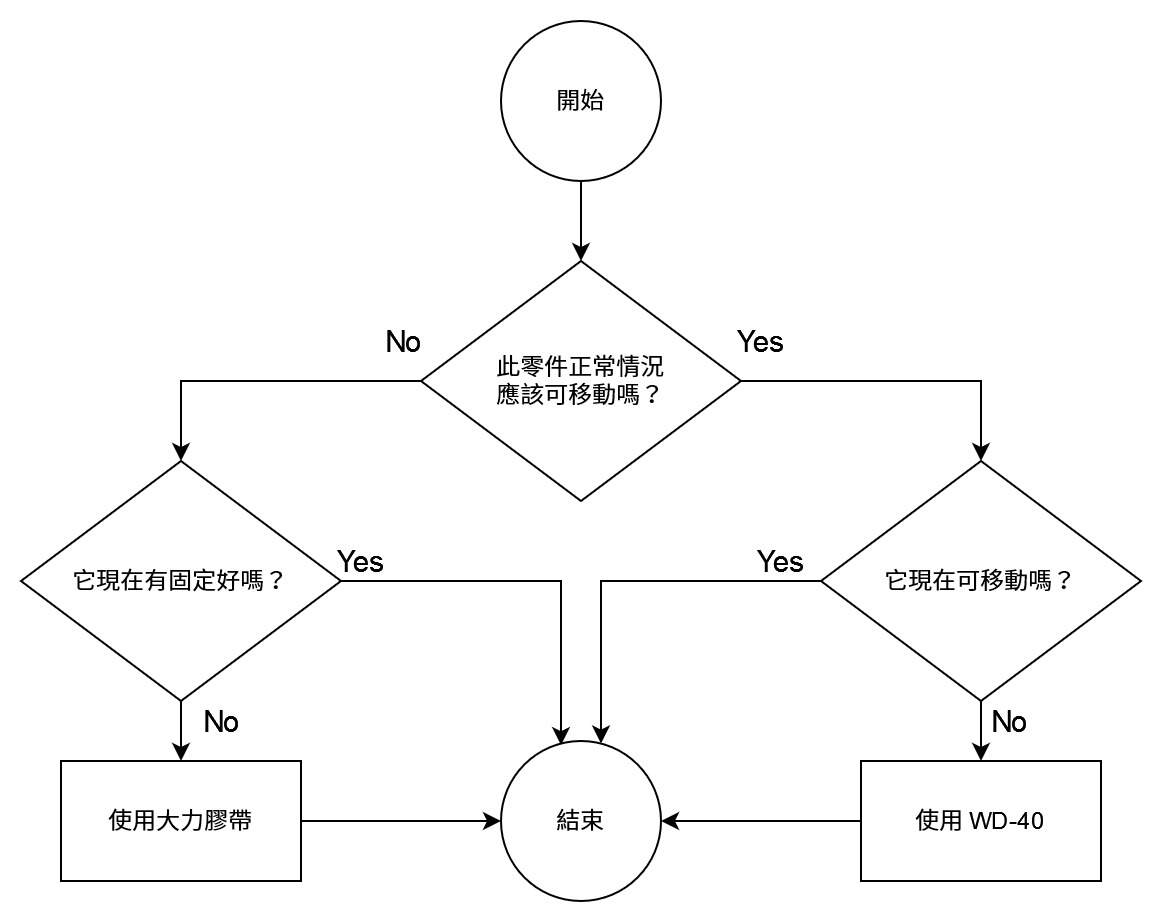
\includegraphics[width=.45\columnwidth]{debug.jpg}} 
\caption{圖片排版}
\label{i:test-fig}

\end{figure}



%% ==================== method ====================
\chapter{研究方法}
\label{c:methoc}
\section{研究設計與流程}

圖\ref{i:debug}顯示了遇到機械機構問題時採用的解法流程圖。
\begin{figure}[!htbp]
\centering

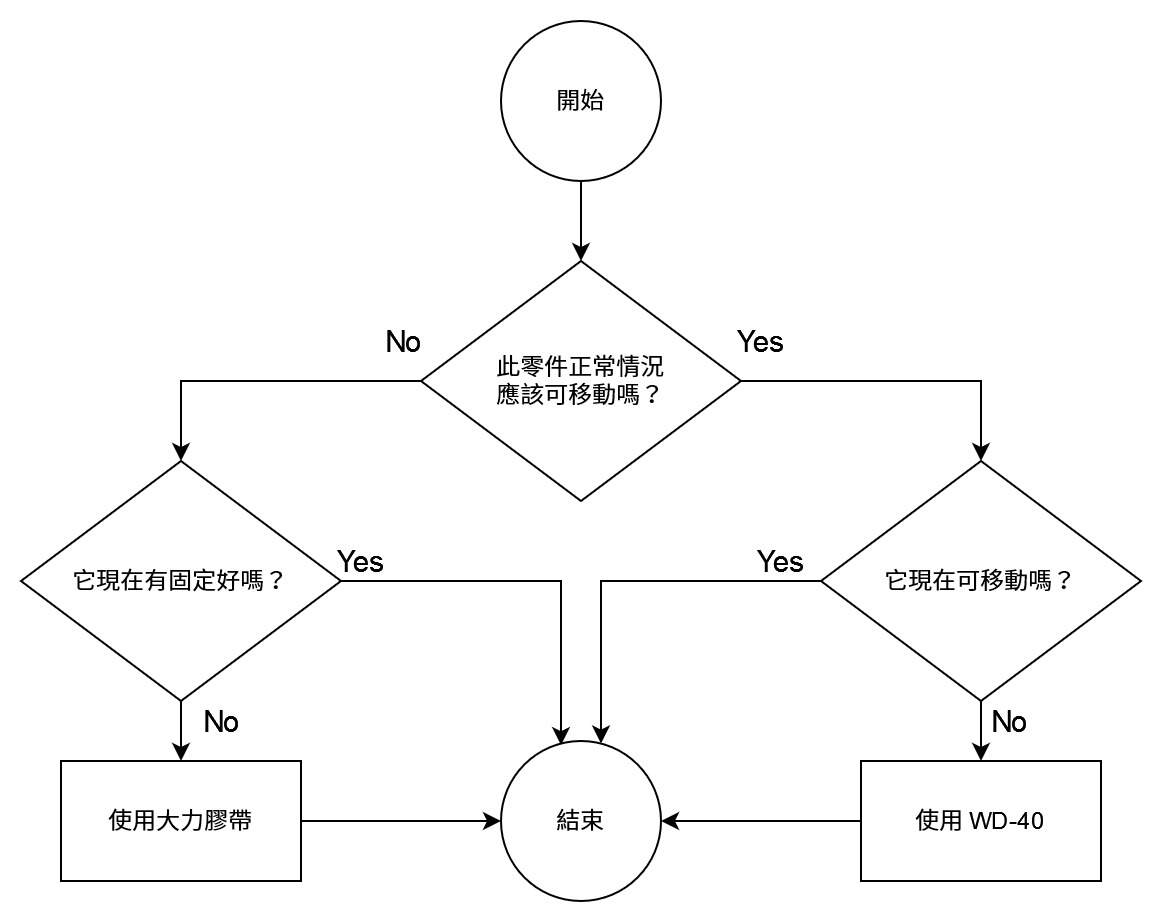
\includegraphics[width=.85\columnwidth]{debug.jpg}
\caption{機械問題除錯流程圖}
\label{i:debug}

\end{figure}


樹範例如~\ref{i:tree}
\begin{figure}[!htbp]
\centering

\tikzset{every tree node/.style={align=center},
    level distance=40pt,
    sibling distance=6pt}
\begin{tikzpicture}
\Tree[.root
       [ (a) ]
       [.node
         [.node
           [ (b) ]
           [ (c) ]
         ]
         [.node
           [ (d) ]
           [ (e) ]
           [ (f) ]
           [ (g) ]
           [ (h) ]
         ]
       ]
     ]

\end{tikzpicture}

\caption{A tree. }
\label{i:tree}
\end{figure}

\clearpage

長條圖範例如~\ref{i:barchart}
\begin{figure}[!htbp]
    \centering
    \vspace{2em}
    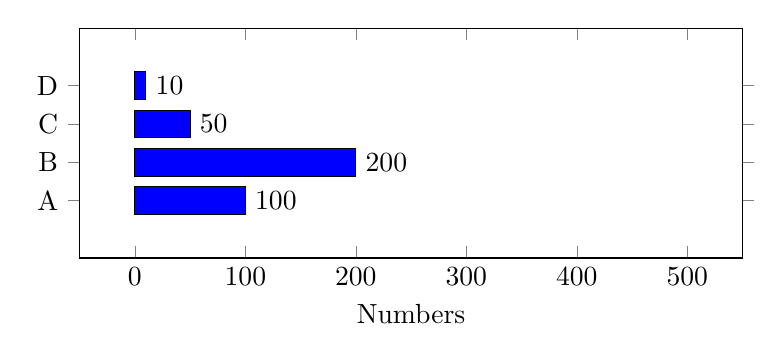
\begin{tikzpicture}
        \begin{axis}[
            enlarge y limits=0.5,
            enlarge x limits=0.1,
            height=4.5cm,
            width=10cm,
            symbolic y coords={A,B,C,D},
            xmin=0,
            xmax=500,
            xbar=1pt,
            xlabel=Numbers,
            nodes near coords={\pgfmathprintnumber[/pgf/number format/assume math mode]{\pgfplotspointmeta}},
            nodes near coords align={horizontal},
            every node near coord/.append style={
                anchor=west}
            ,
            xticklabel style={/pgf/number format/assume math mode},
            yticklabel style={/pgf/number format/assume math mode},
            ytick=data
          ]
            \addplot[xbar,fill=blue] coordinates {
            (100,A)
            (200,B)
            (50,C)
            (10,D)
            };
        \end{axis}
    \end{tikzpicture}
    \caption{A barchart.}
    \label{i:barchart}
\end{figure}



%% ==================== experiment ====================
\chapter{實驗結果}
\label{c:experiment}

\section{描述性統計}

本研究各變數實驗結果之描述性統計(個數、最小值、最大值、平均與標準差)如表~\ref{t:a}。

\begin{table}[htbp]
\centering

\caption{受測者描述性統計}
\label{t:a}

\begin{adjustbox}{max width=0.95\textwidth}
\begin{tabular}{lcccrc} % 對齊

\toprule
變數  & 個數 & 最小值 & 最大值 & 平均數      & 標準差 \\ 
\midrule
背景  & 5   &       &       &  35,856    &       \\
資料A & 84  &       &       &  55        &       \\
資料B & 4   &       &       &  2,033.5   &       \\
\bottomrule
\multicolumn{6}{l}{註：本表的內容僅供參考}

\end{tabular}
\end{adjustbox}
\end{table}


\section{實驗結果分析}

如表~\ref{t:b}，以雙獨立樣本t檢定檢驗...

\begin{table}[htbp]
\centering
\caption{測試(N=50)}
\label{t:b}
\begin{adjustbox}{max width=\textwidth}
\begin{tabular}{@{}ccccclrc@{}}
\toprule
 \multirow{2}[3]{*}{樣本} & \multicolumn{2}{c}{測試一} & \multicolumn{2}{c}{測試二} &  &  &  \\ \cmidrule(lr){2-5}
 & 平均 & 標準差 & 平均 & 標準差 & 自由度 & t值 & \textit{p-value} \\ \midrule
Q1 & 3.58 & 1.64 & 3.23 & 1.84 & 48 & -.71 & .47 \\
Q2 & 3.71 & 1.48 & 4.04 & 1.42 & 48 & .80 & .42 \\
Q3 & 5.46 & 2.22 & 6.15 & 1.51 & 40.126 & 1.28 & .20 \\ \bottomrule
\end{tabular}
\end{adjustbox}
\end{table}

如表~\ref{t:c}所示...

\begin{sidewaystable}

\centering
\caption{測試anova(N=50)}
\label{t:c}
\begin{adjustbox}{max width=\textwidth}
\begin{tabular}{@{}crrrrr@{}}

\toprule
\multicolumn{1}{l}{} & \multicolumn{1}{c}{\begin{tabular}[c]{@{}c@{}}G1\\ 測試\\ N=12\\ (M/SD)\end{tabular}} & \multicolumn{1}{c}{\begin{tabular}[c]{@{}c@{}}G2\\ 測試\\ N=12\\ (M/SD)\end{tabular}} & \multicolumn{1}{c}{\begin{tabular}[c]{@{}c@{}}G3\\ 測試\\ N=14\\ (M/SD)\end{tabular}} & \multicolumn{1}{c}{\begin{tabular}[c]{@{}c@{}}G4\\ 測試\\ N=12\\ (M/SD)\end{tabular}} & \multicolumn{1}{c}{\begin{tabular}[c]{@{}c@{}}F\\ (df)\end{tabular}} \\
\midrule
\multicolumn{1}{l}{變數名稱} & \multicolumn{1}{c}{} & \multicolumn{1}{c}{} & \multicolumn{1}{c}{} & \multicolumn{1}{c}{} & \multicolumn{1}{c}{} \\
測試 & (7.25/1.76) & (6.00/1.80) & (6.43/1.91) & (6.42/1.73) & \begin{tabular}[c]{@{}r@{}}1.00\\ (3,46)\end{tabular} \\
測試 & (40.16/12.01) & (40.08/11.13) & (34.35/10.93) & (36.33/7.66) & \begin{tabular}[c]{@{}r@{}}.95\\ (3,46)\end{tabular} \\
測試 & (68.83/14.04) & (68.83/23.37) & (79.21/22.73) & (81.75/30.13) & \begin{tabular}[c]{@{}r@{}}1.05\\ (3,46)\end{tabular} \\
測試 & (39.25/74.65) & (10.66/91.36) & (30.71/38.42) & (18.00/90.86) & \begin{tabular}[c]{@{}r@{}}.19\\ (3,46)\end{tabular} \\
測試 & (1.37/.42) & 高(1.58/.82) & (1.11/.62) & 低(.80/.63) & \begin{tabular}[c]{@{}r@{}}3.33*\\ (3,46)\end{tabular} \\
測試 & (04.66/12.66) & (39.83/11.26) & (71.92/29.64) & (39.50/19.43) & \begin{tabular}[c]{@{}r@{}}.71\\ (3,46)\end{tabular} \\
測試 & (4.84/1.21) & (5.14/1.41) & (4.59/1.12) & (4.78/1.45) & \begin{tabular}[c]{@{}r@{}}.40\\ (3,46)\end{tabular} \\
測試 & (10.45/34.43) & (05.12/41.36) & (87.46/34.60) & (95.20/30.74) & \begin{tabular}[c]{@{}r@{}}1.08\\ (3,46)\end{tabular} \\
\bottomrule
\end{tabular}
\end{adjustbox}

\end{sidewaystable}


%% ==================== conclusion ====================
\chapter{結論與建議}
\label{c:conclusion}

\section{實驗結果討論}

測試文字測試文字測試文字測試文字測試文字測試文字測試文字測試文字測試文字測試文字測試文字測試文字測試文字測試文字測試文字測試文字

\subsection{綜合討論}

測試文字測試文字測試文字測試文字測試文字測試文字測試文字測試文字測試文字測試文字測試文字測試文字測試文字測試文字測試文字測試文字

\section{其他實驗結果討論}

\section{總結與未來建議}

引述甘道夫（Gandalf）之名言——You shall not pass。

\section{研究限制}


%% ── 參考文獻 ────────────────────────────────────────────────────────────
\clearpage
\phantomsection
\addcontentsline{toc}{chapter}{\bibname}
\bibliographystyle{ieeetr}
\bibliography{thesis}

%% ── 附錄 ────────────────────────────────────────────────────────────────
\NFUAppendix
\clearpage
\chapter{附錄一}
\label{appendix}

根據文獻\cite{nfu2021}製作本樣板。

\vspace{1.5cm}

尤拉恆等式（Euler's identity）被理察·費曼（Richard Feynman）喻爲「最美的公式」：
\begin{Large}
\begin{equation}
    e^{i \pi} + 1 = 0 \label{euler-identity}
\end{equation}
\end{Large}

\vspace{1.5cm}

PID控制器可以表示為式\eqref{pid}。其中$e$為誤差，定義為目標設定值減去實際回授值：$e=V_{exp}-V_{act}$。

\begin{equation}
    u(t) = \underbrace{K_p e(t)}_{\rm P-term}
         + \underbrace{K_i \int_{0}^{t} e(\tau)\mathrm{d}\tau}_{\rm I-term}
         + \underbrace{K_d \frac{\mathrm{d}}{\mathrm{d}t} e(t)}_{\rm D-term}
    \label{pid}
\end{equation}

\vspace{1.5cm}

\begin{align}
^{base}\mathbf{T}_{end} &= \; ^0\mathbf{T}_2 = \; ^0\mathbf{T}_1 \; ^1\mathbf{T}_2 \\
&=
\begin{bmatrix}
\cos \theta_1&0&\sin \theta_1&0\\
\sin \theta_1&0&-\cos \theta_1&0\\
0&1&0&0\\
0&0&0&1
\end{bmatrix}
\begin{bmatrix}
\cos \theta_2&-\sin \theta_2&0&l_1\cos \theta_2\\
\sin \theta_2&\cos \theta_2&0&l_1\sin \theta_2\\
0&0&1&d_2\\
0&0&0&1
\end{bmatrix}
\end{align}

\begin{align}
sign(x) =
\left\{
    \begin{array}{rl}
    1, & x>0 \\
    0, & x=0 \\
    -1, & x<0
    \end{array}
\right.
\end{align}

\vspace{1.5cm}

上下標：$^1_2x^3_4$

\clearpage
善用 "clearpage" 來排版，特別是圖表的分佈。


%% ── 英文論文大綱 ────────────────────────────────────────────────────────
\begin{NFUExtendedAbstract}

% 這部分的格式處理的不是很好，若有問題的話，也可以用其他軟體打完輸出成 PDF 檔
% 再於 “thesis.tex” 使用 "\includepdf[pages={1}, pagecommand={}]{pdfs/XXX.pdf}" 來插入 PDF。 



The extended abstract should be approximately 3-5 pages in length (including references, tables and figures). It should be written in English using font Times New Roman size 12 pt. Manuscript should be divided into sections: Abstract, Keywords, Introduction, Materials \& Methods, Results \& Discussion and References. 
\\

\noindent
Keywords: test, test, test, test, test

\clearpage % 換頁

% \section{Introduction}
{\fontsize{16}{18}\selectfont
\noindent
\textbf{1. Introduction}}\\
\vspace{-2em}

Testtesttesttesttesttesttesttesttesttest, testesttestttesttest, testtesttesttest. Testtesttesttesttesttesttest, testtesttest.

Testtesttesttesttesttesttest.

\vspace{2em}
{\fontsize{16}{18}\selectfont
\noindent
\textbf{2. Review}}\\
\vspace{-2em}

Testtesttesttesttesttesttest.

\vspace{2em}
{\fontsize{16}{18}\selectfont
\noindent
\textbf{3. Method}}\\
\vspace{-2em}

Testtesttesttesttesttesttest.

\vspace{2em}
{\fontsize{16}{18}\selectfont
\noindent
\textbf{4. Experiment}}\\
\vspace{-2em}

Testtesttesttesttesttesttest.

\vspace{2em}
{\fontsize{16}{18}\selectfont
\noindent
\textbf{5. Conclusion}}\\
\vspace{-2em}

Testtesttesttesttesttesttest.



\end{NFUExtendedAbstract}

\end{document}
